\documentclass{article}
\usepackage[a4paper, portrait, margin=1.1811in]{geometry}
\usepackage[dvipsnames]{xcolor}
\usepackage[english]{babel}
\usepackage[utf8]{inputenc}
\usepackage[T1]{fontenc}
\usepackage{helvet}
\usepackage{pgf-umlsd}
\usepackage{etoolbox}
\usepackage{amsfonts}
\usepackage{enumitem}
\usepackage{graphicx}
\usepackage{titlesec}
\usepackage{caption}
\usepackage{booktabs}
\usepackage{adjustbox}
\usepackage{subcaption}
\usepackage{multicol}
\usepackage{float}
\usepackage{amsmath}
\usepackage{listings}
\usepackage{tikz}
\usepackage[colorlinks, citecolor=cyan]{hyperref}

\usetikzlibrary{matrix,shapes,arrows,positioning,chains, calc}
\definecolor{dkgreen}{rgb}{0,0.6,0}
\definecolor{gray}{rgb}{0.5,0.5,0.5}
\definecolor{mauve}{rgb}{0.58,0,0.82}

\usepackage{caption}
\captionsetup[figure]{labelfont={bf},labelformat={default},labelsep=period,name={Figure }}	
% \captionsetup[table]{labelfont={bf},labelformat={default},labelsep=period,name={Table }}
\graphicspath{ {./images/} }
\usepackage{scrextend}
\usepackage{fancyhdr}
\usepackage{graphicx}
\newcounter{lemma}
\newtheorem{lemma}{Lemma}
\newcounter{theorem}
\newtheorem{theorem}{Theorem}

\fancypagestyle{plain}{
	\fancyhf{}
	\renewcommand{\headrulewidth}{0pt}
	\renewcommand{\familydefault}{\sfdefault}
	
}

%\pagestyle{plain}
\makeatletter
\setlength{\@fptop}{0pt}
\patchcmd{\@maketitle}{\LARGE \@title}{\fontsize{16}{19.2}\selectfont\@title}{}{}
\makeatother

\usepackage{authblk}
\def\code#1{\texttt{#1}}
\renewcommand\Authfont{\fontsize{10}{10.8}\selectfont}
\renewcommand\Affilfont{\fontsize{10}{10.8}\selectfont}
\renewcommand*{\Authsep}{, }
\renewcommand*{\Authand}{, }
\renewcommand*{\Authands}{, }
\setlength{\affilsep}{2em}  
\newsavebox\affbox
\author[1]{\textbf{Aarav Varshney}}
% \author[2]{\textbf{Mahabir Prasad Jhanwar}}
\affil[1]{\textbf{Ashoka University}, \texttt{aarav.varshney@alumni.ashoka.edu.in}}
% \affil[2]{\textbf{Ashoka University}, \texttt{mahavir.jhawar@ashoka.edu.in}
% }

\titlespacing\section{0pt}{12pt plus 4pt minus 2pt}{0pt plus 2pt minus 2pt}
\titlespacing\subsection{12pt}{12pt plus 4pt minus 2pt}{0pt plus 2pt minus 2pt}
\titlespacing\subsubsection{12pt}{12pt plus 4pt minus 2pt}{0pt plus 2pt minus 2pt}


\titleformat{\section}{\normalfont\fontsize{10}{15}\bfseries}{\thesection.}{1em}{}
\titleformat{\subsection}{\normalfont\fontsize{10}{15}\bfseries}{\thesubsection.}{1em}{}
\titleformat{\subsubsection}{\normalfont\fontsize{10}{15}\bfseries}{\thesubsubsection.}{1em}{}

\titleformat{\author}{\normalfont\fontsize{10}{15}\bfseries}{\thesection}{1em}{}

\title{\textbf{\huge Report on TLS 1.3}\\}
\date{}    

\begin{document}

\pagestyle{headings}	
\newpage
\setcounter{page}{1}
\renewcommand{\thepage}{\arabic{page}}

\setlength{\parskip}{0.5em}
	
\maketitle
	
\noindent\rule{15cm}{0.5pt}
	\begin{abstract}
        The Internet Engineering Task Force (IETF) formed the Transport Layer Security (TLS) working group to develop a standardized SSL-like protocol. In 1999, the group released the specification for the TLS 1.0 protocol \cite{rfc793}, which is a minor variation of SSL 3.0 and is sometimes referred to as SSL version 3.1. In 2006 and 2008, minor updates were made to TLS 1.0, leading to the development of TLS version 1.2. However, due to numerous security vulnerabilities, TLS 1.2 was overhauled in 2017, resulting in the much stronger TLS version 1.3 \cite{rfc8446}. TLS has become widely used in software systems worldwide. This report will mostly focus on TLS 1.3.
	\end{abstract}
\noindent\rule{15cm}{0.4pt}

\section{Introduction}

\begin{figure}[H]
    \centering
    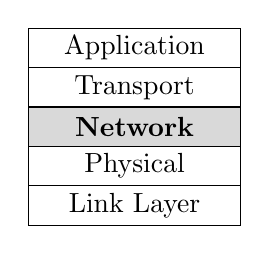
\begin{tikzpicture}[node distance=0 cm,outer sep = 0pt,inner sep = 2pt]
        \tikzset{field/.style={align=center,shape=rectangle,minimum height=0.5cm,minimum width=9mm,draw}}
        \tikzset{largefield/.style={align=center,shape=rectangle,minimum height=0.5cm,minimum width=27mm,draw}}
    
        \node [largefield] (application) {Application};
        % \node [field,right=of tor] (vpn) {VPN};
        % \node [field,right=of vpn] {\dots};
    
        \node [largefield,below=of application] (transport) {Transport};
        \node [largefield,below=of transport,fill=gray!30] (network) {\textbf{Network}};
        \node [largefield,below=of network] (phys) {Physical};
        \node [largefield,below=of phys] {Link Layer};
    \end{tikzpicture}
    
    \caption{The TCP/IP Reference Model \cite{tcpip}}
    \label{fig:tcpip}
    \hrulefill
\end{figure}

When two computers want to send data to each other, they may use the \textbf{Internet Protocol} (IP) \cite{rfc791} directly. IP fragments data into blocks of data called \textit{packets} (also called datagrams) and transmits them from the source to the destination. The sources and destinations are computers identified by fixed length addresses. However, IP is a low-level protocol that does not interact directly with application data and may cause unreliable data transmission.

In the TCP/IP Reference Model \cite{tcpip}, the IP protocol works in the network layer, which is two layers below the application layer (see Figure \ref{fig:tcpip}). This layer provides an unreliable, connectionless delivery system (there is no direct connection between two hosts) which does not provide any functionality for error recovery for datagrams that are either duplicated, lost or arrive at the remote host in another order than they were sent. The transport layer, which is the layer above the network layer, is responsible for fixing the unreliable data transmission with transport protocols like \textbf{Transmission Control Protocol (TCP)} \cite{rfc793}. TCP is the most commonly used transport protocol on top of IP and includes strategies for packet ordering, retransmission, and maintaining data integrity.

TCP is a connection-oriented protocol, which means that before any data can be sent, a connection must be established between the two hosts. This connection is established by a three-way handshake between the two hosts. The first computer sends a packet with the SYN (a field in the TCP header) bit set to 1. The second computer responds with a packet with the SYN and ACK (another field in the TCP header) bits set to 1. The first computer then sends a packet with the ACK bit set to 1. Once the connection is established, the two hosts can start sending data to each other.

Now that we have established a connection between two hosts and have the ability to reliably send data across, we can further improve the transmission by using \textbf{Transport Layer Security (TLS)} \cite{rfc8446} (original \cite{rfc2246}). TLS protocol allows two hosts to communicate in a way that is designed to prevent eavesdropping, tampering, or message forgery. While TCP provides reliable data transmission, the data in the packets is unencrypted and can be read by anyone who has access to the network. This is acceptable when the data is not sensitive, but when the data is sensitive, TLS is used to \textit{encrypt} the data. TLS also provides \textit{authentication} of the remote host, which means that the remote host can be trusted to be the host it claims to be.

TLS is primarily used in a client/server setting where the client initiates the connection and the server responds. Setting up a TLS connection requires a handshake between the client and the server. At the end of the handshake, the client and the server have agreed upon a shared secret key which is used to encrypt the data, the encryption schemes and their parameters, and the client is also assured of the server's identity (not without issues \cite{rfc6962, tlsCertificateIssues}).

In this report, we discuss TLS 1.3 \cite{rfc8446}, which is the latest version of TLS in two sections. Section 1 covers the \textit{handshake protocol} in TLS 1.3. Section 2 discusses the \textit{record protocol} that uses the parameters established by the handshake protocol to protect traffic between the communicating hosts.



\section{Background}
\label{sec:background}
\subsection{Authenticated Encryption (AE)}
Cryptographic applications commonly require both confidentiality and message authentication. Confidentiality ensures that data is available only to those authorized to obtain it; usually it is realized through encryption.  Message authentication is the service that ensures that data has not been altered or forged by unauthorized entities; it can be achieved by using a Message Authentication Code (MAC). This service is also called data integrity. \textbf{Authenticated Encryption (AE)} \cite{ae} schemes ensure both data secrecy (confidentiality) and data integrity. These schemes can be constructed with either a \textbf{generic composition} that combines a CPA-secure cipher with a secure MAC, or to build them directly from a block cipher or a PRF without first constructing either a standalone cipher or MAC \cite{gradcourse}. The latter schemes are called \textbf{integrated schemes}.

Let $(E, D)$ be a cipher and $(S, V)$ be a MAC. Let $k_{enc}$ be a cipher key and $k_{mac}$ be a MAC key. In a generic composition, these two primitives can be combined using two commonly used options: \textbf{Encrypt-then-MAC} and \textbf{MAC-then-Encrypt}. In the first option, the plaintext is encrypted using the cipher and the resulting ciphertext is authenticated using the MAC. In the second variant, the plaintext is first authenticated using the MAC and the resulting MAC tag along with the plaintext is encrypted using the cipher (see Figure \ref{fig:encrypt-then-mac} and Figure \ref{fig:mac-then-encrypt}). Only the first method is secure for every combination of CPA-secure cipher and secure MAC. The intuition is that the MAC on the ciphertext prevents any tampering with the ciphertext. The second method is known to have attacks in some cases \cite{gradcourse}.

\subsection{Authenticated Encryption with Associated Data (AEAD)}
TLS uses a nonce-based \textbf{Authenticated Encryption with Associated Data (AEAD)} \cite{aead} cipher to encrypt and authenticate packets. AEAD schemes are an extension of AE schemes (discussed above) that adds the ability to check the integrity and authenticity of some Associated Data (AD), also called "additional authenticated data", that is not encrypted. The associated data is required to set context; for example in a networking protocol, authenticated encryption protects the packet body, but the header must be transmitted in the clear so that the network can route the packet to its intended destination \cite{gradcourse}. Nonetheless, we want to ensure header integrity so that a malicious adversary can't get away with tampering the header. This header is provided as the associated data input to the AEAD encryption scheme. Secondly, the encryption scheme takes an additional input nonce $\mathcal{N}$, which is a random value that is used only once. This nonce ensures that the same plaintext is never encrypted to the same ciphertext. The nonce can be kept with the encrypted message or created just before it's decrypted. The decryption process only needs enough information to reconstruct the nonce. For example, a system could use a nonce consisting of a sequence number in a particular format, in which case it could be inferred from the order of the ciphertexts. If a wrong nonce is used, the decryption process will still detect it as incorrect, so it won't compromise security.

The interface to the AEAD is relatively simple, since it requires only a single key as input and requires only a single identifier to indicate the algorithm in use in a particular case unlike AE where you have to specify the combination of cipher and MAC. The authenticated encryption operation has four inputs, each of which is an octet string:
\begin{enumerate}
  \item A secret key K, which MUST be generated in a way that is uniformly
        random or pseudorandom.
  \item A nonce $\mathcal{N}$. Each nonce provided to distinct invocations of the
        Authenticated Encryption operation MUST be distinct, for any particular value of the key, unless each and every nonce is zero-
        length.
  \item A plaintext P, which contains the data to be encrypted and authenticated.
  \item The associated data A, which contains the data to be authenticated, but not encrypted.
\end{enumerate}
The output is a ciphertext C, which is at least as long as the plaintext.
% \newpage
\begin{figure}[t]
  \centering
  \begin{subfigure}[b]{0.4\textwidth}
    \centering
    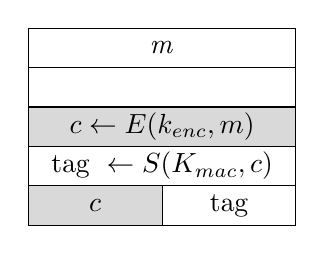
\begin{tikzpicture}[node distance=0 cm,outer sep = 0pt,inner sep = 2pt]
      \tikzset{field/.style={align=center,shape=rectangle,minimum height=0.5cm,minimum width=17mm,draw}}
      \tikzset{largefield/.style={align=center,shape=rectangle,minimum height=0.5cm,minimum width=34mm,draw}}

      \node [largefield] (message) {\textit{m}};
      \node [largefield, below=of message] (empty) { };
      \node [largefield,below=of empty,fill=gray!30] (enc) {$c \leftarrow E(k_{enc}, m)$};
      \node [largefield,below=of enc] (mac) {$\text{tag } \leftarrow S(K_{mac}, c)$};
      \node [field,below=of mac, xshift=-8.5mm, fill=gray!30] (cipher) {$c$};
      \node [field,below=of mac, xshift=8.5mm] (tag) {tag};
    \end{tikzpicture}
    \caption{Encrypt-then-MAC}
    \label{fig:encrypt-then-mac}
  \end{subfigure}
  \begin{subfigure}[b]{0.4\textwidth}
    \centering
    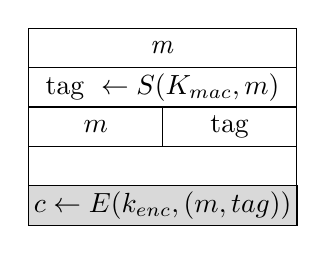
\begin{tikzpicture}[node distance=0 cm,outer sep = 0pt,inner sep = 2pt]
      \tikzset{field/.style={align=center,shape=rectangle,minimum height=0.5cm,minimum width=17mm,draw}}
      \tikzset{largefield/.style={align=center,shape=rectangle,minimum height=0.5cm,minimum width=34mm,draw}}

      \node [largefield] (message) {\textit{m}};
      \node [largefield,below=of message] (mac) {$\text{tag } \leftarrow S(K_{mac}, m)$};
      \node [field,below=of mac, xshift=-8.5mm] (pkt-m) {$m$};
      \node [field,below=of mac, xshift=8.5mm] (tag) {tag};
      \node [largefield, below=of pkt-m, xshift=8.5mm] (empty) { };
      \node [largefield,below=of empty,fill=gray!30] (enc) {$c \leftarrow E(k_{enc}, (m, tag))$};

    \end{tikzpicture}
    \caption{MAC-then-Encrypt}
    \label{fig:mac-then-encrypt}
  \end{subfigure}
  \label{fig:encrypt-then-mac-mac-then-encrypt}
  \caption{Two different ways to combine a cipher and a MAC.}
  \hrulefill
\end{figure}

\subsection{HMAC-based Extract-and-Expand Key Derivation Function (HKDF)}
The TLS handshake establishes one or more input secrets which are combined to create the actual working keying material using HKDF which uses HMAC at its core.

Hashed Message Authentication Code (HMAC) \cite{rfc2104} is based on a cryptographic hash function $H : \{0, 1\}^* \rightarrow \{0, 1\}^\lambda$ and keyed with some key $K \in \{0, 1\}^\lambda$ (larger key material is hashed through H to obtain a $\lambda$-bit key). Computing the HMAC value on some message m is then defined as $\textit{HMAC}(K, m) := H((K \oplus \textit{opad}) \mathbin\Vert H((K \oplus \textit{ipad}) \mathbin\Vert m))$, where \textit{opad} and \textit{ipad} are two $\lambda$-bit padding values consisting of repeated bytes 0x5c and 0x36, respectively.

A key derivation function (KDF) is a basic and essential component of cryptographic systems.  Its goal is to take some source of initial keying material and derive from it one or more cryptographically strong secret keys \cite{hdkf}. The main difficulty in designing a KDF relates to the form of the initial keying material. When this key material is given as a uniformly random or pseudorandom key $K$ then one can use $K$ to seed a pseudorandom function (PRF) or pseudorandom generator (PRG) to produce additional cryptographic keys. However, when the source keying material is not uniformly random or pseudorandom then the KDF needs to first ``extract'' from this ``imperfect'' source a first pseudorandom key from which further keys can be derived using a PRF. Thus, one identifies two logical modules in a KDF: a first module that takes the source keying material and extracts from it a fixed-length pseudorandom key K, and a second module that expands K into several additional pseudorandom cryptographic keys. This two-module paradigm is called the ``extract-then-expand'' paradigm. 

The expansion module is standard in cryptography and can be implemented on the basis of any secure PRF. The extraction functionality, in turn, is well modeled by the notion of randomness extractors \cite{hdkf}. There exists computational extractors, namely randomness extractors where the output is only required to be pseudorandom rather than statistically close to uniform. Computational extractors are well-suited for the cryptographic setting where attackers are computationally bounded and source entropy may only exist in a computational sense. KDFs accept four inputs: a sample from the source of keying material from which the KDF needs to extract cryptographic keys, a parameter defining the number of key bits to be output, an (optional) randomizing salt value as mentioned before, and a fourth ``contextual information'' field. The latter is an important parameter for the KDF intended to include key-related information that needs to be uniquely and cryptographically bound to the produced key material (e.g., a protocol identifier, identities of principals, timestamps, etc.) \cite{hdkf}. 

The computation of extract-then-expand KDFs is specified as follows:
\begin{equation}
\label{eq:hdkf1}
\begin{split}
  & \textit{PRK = XTR (XTS, SKM)} \\
  & \textit{KM = PRF*(PRK, CTXinfo, L)}
\end{split}
\end{equation}
  
where \textit{XTR} is the extractor function, \textit{PRF*} is a variable-length output pseudorandom function used in the expansion module, and $L$ is the desired length of the output key material.

HMAC-based key derivation function (HKDF) \cite{hdkf} follows the above mentioned "extract-then-expand" paradigm and uses HMAC as the underlying PRF in both extract and expand modules. HDKF is specified as: 

\begin{equation}
\label{eq:hdkf}
\text{HKDF}(\textit{XTS}, \textit{SKM}, \textit{CTXinfo}, L) = K(1)\mathbin\Vert K(2) \mathbin\Vert . . . \mathbin\Vert K(t)
\end{equation}

where the values $K(i)$ are defined as follows:
\begin{equation}
\label{eq:hdkf2}
\begin{split}
  &PRK = \text{HMAC}(\textit{XTS}, \textit{SKM}) \\
  &K(1) = \text{HMAC}(\textit{PRK}, \textit{CTXinfo} \mathbin\Vert 0) \\
  &K(i + 1) = \text{HMAC}(\textit{PRK}, K(i) \mathbin\Vert \textit{CTXinfo} \mathbin\Vert i) 1 \leq i \le t,
\end{split}
\end{equation}
where $t = \lceil L/k \rceil$  where $k$ denotes the output (and key) length of the hash function used with HMAC and the value $K(t)$ is truncated to its first $d = L \mod k$ bits; the counter $i$ is of a given fixed size, e.g., a single byte. The source key material is \textit{SKM}, the extractor salt is \textit{XTS} (which may be null or constant), the number \textit{L} of key bits to be produced by KDF, and a ``context information'' string \textit{CTXinfo} (which may be null) \cite{hdkf}.

\subsection{TLS 1.3 Key Derivation}
\fbox{\parbox{\textwidth}{The Key Derivation process in TLS 1.3 makes use of the HKDF-Extract and HKDF-Expand functions as well as the functions defined below \cite{rfc8446}:
\begin{itemize}
  \item \textbf{HKDF-Extract}: HKDF-Extract(Salt, IKM) $\rightarrow$ PRK
  \item \textbf{HKDF-Expand}: HKDF-Expand(PRK, Info, L) $\rightarrow$ OKM
  \item \textbf{HKDF-Expand-Label}: HKDF-Expand-Label(Secret, Label, Context, Length) $\rightarrow$ HKDF-Expand(Secret, HkdfLabel, Length)
  \item \textbf{HkdfLabel}: HkdfLabel(Length, Label, Context): (length = Length; label = "tls13 " + Label; context = Context) $\rightarrow$ HkdfLabel
  \item \textbf{Derive-Secret}: Derive-Secret(Secret, Label, Messages) $\rightarrow$ HKDF-Expand-Label(Secret, Label, Transcript-Hash(Messages), Hash.length)
\end{itemize}
}}


\section{TLS Handshake Protocol}
\label{sec:handshake}
For consistency with the notation, we let P play the role of the client and Q play the role of the server. P and Q wish to setup a secure session. 

\textbf{TLS 1.3} supports both one-sided and mutual authentication. In most cases, authentication for the client is optional. In the notation, $(E_s , D_s)$ is a symmetric encryption scheme that provides authenticated encryption, such as AES-128 in GCM mode.  Algorithm $S$ refers to a MAC signing algorithm, such as HMAC-SHA256. Algorithms $Sig_P(\cdot )$ and $Sig_Q(\cdot )$ sign the provided data using P's or Q's signing keys. Finally, the hash functions $H_1, H_2$ are used to derive symmetric keys. They are built from HKDF with hash functions such as SHA-256. 

The cipher-suites which determine the symmetric encryption scheme, the hash function in the MAC signing algorithm and HKDF are negotiated during the handshake. The cipher-suites are defined in \cite{rfc8446}. They are specified in Table \ref{tab:ciphersuites}. TLS negotiates these algorithms, rather than hard code a specific choice, because some organizations may prefer to use different algorithms based on their policies.


\textbf{The protocol.} In the first step \textbf{Client Hello}, P sends a message to Q. The message contains a 32 bytes nonce $\mathcal{N}_c$ generated by a secure random number generator and an ``offer''. The offer specifies the group, a list of the symmetric cipher options supported by the client, specifically the record protection algorithm (including secret key length) and a hash to be used with HKDF, in descending order of client preference. In fact, the client can provide several groups in his offer using a ``supported\_groups'' extension though constrained to be one of several pre-defined groups, which include both elliptic curves and subgroups of finite fields. A ``key\_share'' extension provides corresponding group elements for each group. Clients which desire the server to authenticate itself via a certificate must send the ``signature\_algorithms'' extension which indicates the signature algorithms the client can accept. 

After receiving the first flow, the server Q examines the ``offer'' sent by the client. It verifies that the group (or groups) preferred by the client coincides with the group (or groups) that the server is able and willing to use. It also selects an encryption scheme $(E_s , D_s)$ and a hash function
from the offer that it is willing and able to use, if any. If the server is unable to find a compatible group and encryption/hash schemes, the server may send a special ``retry'' request to the client.

The server now responds with \textbf{Server Hello} containing its own nonce $\mathcal{N}_s$, a ``mode'' message which
indicates the parameter choices (group, encryption/hash scheme) made by the server along with the key share corresponding to the selected group. At this point, the server has enough information to compute the client handshake traffic secret (CHTS) and server handshake traffic secret (SHTS) values, and uses these to derive client and server handshake traffic keys ($tk_{chs}$ and $tk_{shs}$, respectively) \\ The server now begins to encrypt all handshake messages under $tk_{shs}$, and any extensions that
are not required to establish the server handshake traffic key are sent (and encrypted) in the \textbf{EncryptedExtensions} (EE) messages \cite{10.1145/2810103.2813653}.

\begin{table}[t]
  \centering
  \begin{tabular}{|l|l|}
    \hline Description & Value \\
    \hline 
    TLS\_AES\_128\_GCM\_SHA256 & $\{0\times13,0\times01\}$ \\
    \hline TLS\_AES\_256\_GCM\_SHA384 & $\{0\times13,0\times02\}$ \\
    \hline TLS\_CHACHA20\_POLY1305\_SHA256 & $\{0\times13,0\times03\}$ \\
    \hline TLS\_AES\_128\_CCM\_SHA256 & $\{0\times13,0\times04\}$ \\
    \hline TLS\_AES\_128\_CCM\_8\_SHA256 & $\{0\times13,0\times05\}$ \\
    \hline
  \end{tabular}
  \caption{Cipher-Suites \cite{rfc8446}. Cipher suite names follow the naming convention: CipherSuite TLS\_AEAD\_HASH = VALUE;}
  \label{tab:ciphersuites}
\end{table}

SHTS/CHTS can be derived as follows \cite{rfc8446}:
% \begin{equation}
%   \label{eq:server_handshake_traffic_secret}
  \begin{verbatim}
  early sercret (ES) =  HKDF-Extract(0, 0)
  derived early secret (dES) = Derive-Secret(ES, "derived", "")
  handshake secret (HS) =  HKDF-Extract(dES, (EC)DHE shared secret)
  SHTS = Derive-Secret(HS, "s hs traffic", ClientHello...ServerHello)
  CHTS = Derive-Secret(HS, "c hs traffic", ClientHello...ServerHello)
  \end{verbatim}
% \end{equation}

The server sends \textbf{EncryptedExtensions} message immediately after the ServerHello message for sending extensions that can be protected. This is followed by \textbf{Certificate Request} message, which is only sent if the server wishes to authenticate the client. If present, this message specifies the type of certificates the server will accept. Finally, the server sends \textbf{Authentication Messages} for authentication, key confirmation (provide explicit proof that an endpoint possesses the private key corresponding to its certificate), and handshake
integrity: \textbf{Certificate}, \textbf{CertificateVerify}, and \textbf{Finished}. All handshake messages in this phase are encrypted under $tk_{shs}$ or $tk_{chs}$. n the full 1-RTT handshake (TODO: Explain 1-RTT and 0-RTT), authentication is based on public key certificates. In pre-shared key handshakes (both PSK and PSK-(EC)DHE), the
server and client will authenticate each other by relying on a message authentication code applied to the transcript. (TODO: This part needs clarity)
\begin{itemize}
  \item ServerCertificate(SV): The server's certificate, and any supporting certificates in the chain.
  
  \item ServerCertificateVerify(SCV): A signature over the value  Transcript-Hash \footnote{Transcript-Hash is computed by hashing the concatenation of each included handshake message, including the handshake message header carrying the handshake message type and length fields, but not including record layer headers \cite{rfc8446}.}(Handshake Context, Certificate). Here, Handshake Context consists of \code{ClientHello}, \code{ServerHello},\\ \code{EncryptedExtensions}, and \code{CertificateRequest} (the conversation so far) using server's signing key. 

 \item ServerFinished(SF): This is the final message in the Authentication Messages. It is essential for providing authentication of the handshake and of the computed keys. The server first derives a server finished key $fk_S$ from SHTS and then computes a MAC tag SF over \code{Transcript-Hash(Handshake Context,Certificate, CertificateVerify)}. This value is also encrypted under $tk_{shs}$, sending the output ciphertext to the client. At this point, the server is able to compute the client application traffic secret (CATS), the server application traffic secret (SATS), and the exporter master secret (EMS).  It can now compute the client application traffic key $tk_{capp}$ and the server application traffic key $tk_{sapp}$ and it can begin sending encrypted application data to the client.
 \begin{equation}
  fk_S = \code{HKDF-Expand-Label(SHTS, ``finished'', '', Hash.length)}
 \end{equation}

 We can derive the traffic keys as follows:
  \begin{equation}
    \label{eq:traffic_keys}
    \begin{split}
      \code{dHS} &= \code{Derive-Secret(HS, "derived", "")} \\
      \code{MS} &= \code{HKDF-Extract(dHS, 0)} \\
      \code{CATS} &= \code{Derive-Secret(MS, "c ap traffic", ClientHello...Server Finished)} \\
      \code{SATS} &= \code{Derive-Secret(MS, "s ap traffic", ClientHello...Server Finished)} \\
      tk_{capp} &= \code{HKDF-Expand-Label(CATS, "key", "", key\_length)} \\
      tk_{sapp} &= \code{HKDF-Expand-Label(SATS, "key", "", key\_length)} 
    \end{split}
  \end{equation}
  \end{itemize}

  \textbf{Client verification, authentication, key confirmation, and key derivation}. The client P,
  upon receiving these messages, checks that the signature SCV (if in full 1-RTT mode) and the  MAC SF verify correctly. If the server Q has requested client authentication, P will begin by sending its digital certificate (carrying its public-key) in the \code{ClientCertificate} message, after which P will compute its own certificate verify value \code{ClientCertificateVerify} by signing the session hash, then send it to Q as the \code{CertificateVerify} message. P finally derives the client finished key $fk_C$ from CHTS and uses $fk_C$ to compute a MAC tag CF over the session hash.

  \textbf{Server verification}. The server will verify the final MAC (CF) and optional signature (CCV) messages of the client.

  \textbf{Handshake completion.} At this point both parties can compute the resumption master secret (RMS) value that can be used as a pre-shared key for session resumption in the future. Both parties can now derive the client application traffic key ($tk_{capp}$), and use the record layer for encrypted communication of application data with the resulting keys.
  \begin{equation}
    RMS = \code{Derive-Secret(MS, "res master", ClientHello...Client Finished)}
  \end{equation}





% \begin{align*}
%     & \textbf { ClientHello } \\
%     & u:=g^\alpha, \mathcal{N}_{\mathrm{c}}, offer \\
%     & \textbf { ServerHello } \\
%     & v:=g^\beta, \mathcal{N}_{\mathrm{s}}, \text { mode } \\ 
%     & c_1:=E_{\mathrm{s}}\left(k_{\mathrm{sh}}, \text { CertReqest }\right) \\ 
%     & c_2:=E_{\mathrm{s}}\left(k_{\mathrm{sh}}, \operatorname{Cert}_Q\right) \\ 
%     & c_3:=E_{\mathrm{s}}\left(k_{\mathrm{sh}}, \text { Sig }\right. \\ 
%     & \left.c_4\left(u, \mathcal{N}_{\mathrm{c}}, \text { offer }, v, \mathfrak{N}_{\mathrm{s}}, \text { mode }, c_1, c_2\right)\right) \\ 
%     & c_4=E_{\mathrm{s}}\left(k_{\mathrm{sh}}, S\left(k_{\mathrm{sm}},\left(u, \mathfrak{N}_{\mathrm{c}}, \text { offer }, v, \mathfrak{N}_{\mathrm{s}}, \text { mode }, c_1, c_2, c_3\right)\right)\right) \\
%     & \left(k_{\mathrm{sh}}, k_{\mathrm{sm}}, k_{\mathrm{ch}}, k_{\mathrm{cm}}\right):=H_1\left(g^{\alpha \beta}, u, \mathcal{N}_{\mathrm{c}}, \text { offer }, v, \mathcal{N}_{\mathrm{s}}, \text { mode }\right) \\
%     & \left(k_{\mathrm{c} \rightarrow \mathrm{s}}, k_{\mathrm{s} \rightarrow \mathrm{c}}\right):=H_2\left(g^{\alpha \beta}, u, \mathcal{N}_{\mathrm{c}}, \text { offer, } v, \mathfrak{N}_{\mathrm{s}}, \text { mode }, c_1, \ldots, c_4\right) \\
%     & \text { ClientKeyExchange } \\
% \end{align*}


\section{TLS Record Protocol}
\label{sec:record}
The TLS record protocol \cite{rfc8446} protects traffic between peers using parameters established by the handshake protocol. Each data packet is referred to as a record, containing a header and a payload. The header includes record type, protocol version, and payload length, while the payload contains the actual data being sent.

TLS defines a Record Layer to receive uninterpreted data from higher layers in non-empty blocks of arbitrary size \cite{rfc2246}. This layer fragments information blocks into \code{TLSPlaintext} records with data chunks of $2^{14}$ bytes or less. There are four record types: \code{ChangeCipherSpec}, \code{Alert}, \code{Handshake}, and \code{ApplicationData}.

The \code{ChangeCipherSpec} record, now deprecated, is used to change the cipher suite used for encryption. The \code{Alert} record is used to send error messages. The \code{Handshake} record is used to send handshake messages, while the \code{ApplicationData} record is used to send application data.

Delignat-Lavaud et al \cite{7958593} argue that each sub-protocol of TLS defines its own data stream, and the record layer is responsible for multiplexing all of these streams into one corresponding to network messages after fragmentation, formatting, padding, and optional record-layer encryption (application data is compulsorily encrypted). According to this model, the record layer is the exclusive user for all non-exported keys generated by the handshake. 

The record protection functions by translating a \code{TLSPlaintext} structure into a \code{TLSCiphertext} structure \cite{rfc8446}. \code{TLSCiphertext} (encrypted record) consists of a plaintext header followed by an encrypted body, which itself contains a type and optional padding.

As per new changes in TLS 1.3, the record layer protection is improved by adopting a single AEAD mode for all ciphersuites, thus deprecating all legacy modes (MAC-only, MAC-pad-encrypt, encrypt-then-MAC \cite{rfc7366}, compress-then-encrypt) \cite{7958593}. The new AEAD mode is designed to be provably-secure and modular, supporting algorithms such as AES-GCM, AES-CCM, and ChaCha20-Poly1305 within the same framework. Recall that AEAD algorithms take as input a single key, a nonce, a plaintext, and ``additional data'' to be included in the authentication check. The key is either of the traffic key generated in \ref{eq:traffic_keys}, the nonce is derived from the sequence number and the \code{client write iv ($iv_{capp}$)} or \code{server write iv ({$iv_{sapp}$)}}, and the additional data input is the record header.

The IVs are generated as follows: 
\begin{equation}
    \begin{split}
        iv_{capp} &= \code{HKDF-Expand-Label(CATS, "iv", "", iv\_length)}\\
        iv_{sapp} &= \code{HKDF-Expand-Label(SATS, "iv", "", iv\_length)}
    \end{split}
\end{equation}

\begin{verbatim}
    additional_data = TLSCiphertext.opaque_type ||
                        TLSCiphertext.legacy_record_version ||
                        TLSCiphertext.length
\end{verbatim}
Here, \code{opaque\_type} is always set to 23 for outward
compatibility with middleboxes accustomed to parsing previous
versions of TLS. The \code{legacy\_record\_version} field is always 0x0303. Finally, the \code{length} (in bytes) of the ecnrypted record. 

A 64-bit sequence number is maintained separately for reading and writing records \cite{rfc8446}. The appropriate sequence number is incremented by one after reading or writing each record. Each sequence number is set to zero at the beginning of a connection and whenever the key is changed; the first record transmitted under a particular traffic key must use sequence number 0. The padded sequence number is XORed with either the $iv_{capp}$ or $iv_{capp}$ (we may use handshake traffic ivs and keys in case of handshake messages). This resulting value is used as the per-record nonce for the AEAD algorithm.
\section{Packet Capture}
We captured a TLS packet sent Facebook. This packet contains to ClientHello message described in Handshake Protocol section. The yellow highlight marks the beginning of the TLS packet with 16 marking the record layer content type as Handshake. The cyan highlighted portion is the random nonce sent by the client to the server. The blue highlights the ciphersuites the client can use to for symmetric encryption.
\begin{figure}[h!]
    \includegraphics*[width=\textwidth]{images/clientHello.png}
\end{figure}
% \section{Applications}
% \input{sections/04_applications.tex}

\newpage
\bibliographystyle{IEEEtran}
\bibliography{bibliography.bib}

\end{document}